\documentclass[12pt, letterpaper]{article}
\usepackage{amsmath}
\usepackage{pgfplots}
\pgfplotsset{compat=1.17}
\usepackage{graphicx} % Required for inserting images

\title{16 Mean-Value Theorem}
\author{Damiam Alfaro}
\date{December 13th 2023}

\begin{document}

\maketitle

\section{The Mean Value Theorem}
\textbf{Motivation}: There is a useful and interesting connection between instantaneous and average rates of change.\\
\newline
\textbf{Goal}: Understand why a differentiable function on an interval has an input value for which the instantaneous rate of change equals the average rate of change over the interval.\\
\newline
\textbf{Rolle's Theorem}: Let \(f\) be continuous on a closed interval \([a,b]\). If \(f(b) = f(a)\), then there is a number \(c\) between \(a\) and \(b\), such that \(f'(c)=0\). The theorem only guarantees the existence of an input value \(c\) in \((a,b)\) at which the derivative is zero. It does not ensure it is unique nor it says how to find it.
\begin{center}
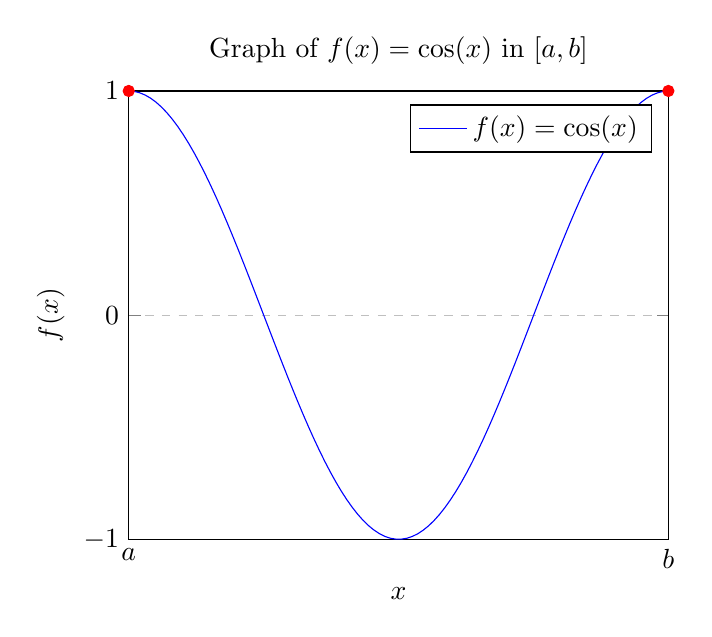
\begin{tikzpicture}
\begin{axis}[
    title={Graph of \( f(x) = \cos(x) \) in \([a, b]\)},
    xlabel={$x$},
    ylabel={$f(x)$},
    xmin=0, xmax=6.28, % 2*pi in terms of decimal
    ymin=-1, ymax=1,
    xtick={0,6.28},
    xticklabels={$a$, $b$},
    ytick={-1, 0, 1},
    legend pos=north east,
    ymajorgrids=true,
    grid style=dashed,
]

% Plotting the function
\addplot[
    domain=0:6.28, % 2*pi in terms of decimal
    samples=100, 
    color=blue,
    ]
    {cos(deg(x))};
\addlegendentry{\( f(x) = \cos(x) \)}

% Indicating the points f(a) and f(b)
\addplot[mark=*,color=red] coordinates {(0,1)};
\addplot[mark=*,color=red] coordinates {(6.28,1)};

\end{axis}
\end{tikzpicture}
\end{center}
Take for example the following:
\[f(x)=x^2-4x+6\]
\begin{enumerate}
    \item First we find whether \(f\) is continuous in the close interval \([0,4]\), which it is
    \item Second we find whether \(f\) is differentiable within \((0,4)\), which it is
    \item Third, we find out whether \(f(a) = f(b)\), which in this case \(f(0) = 6\) and \(f(4) = 6\)
\end{enumerate}
Now we just find \(c\) by solving for it in \(f'(c) = 0\)
\[f'(c) = 2c-4 \]
\[0 = 2c-4\]
\[4 = 2c\]
\[2 = c\]
\textbf{The Mean Value Theorem}: Let \(f\) be continuous on a closed interval \([a,b]\) and assume that \(f\) is differentiable on \((a,b)\). Then, there is a number \(c\) between \(a\) and \(b\) such that:
\[f'(c)=\frac{f(b)-f(a)}{b-a}\]
The above formula is also the formula for the \underline{average rate of change}:
\[f(b)-f(a)=f'(c)(b-a)\]
There will be times where they will ask you to estimate \(f(b)-f(a)\) without giving you a function, just an interval for the function \(f\) and an interval for its derivative \(f'(x)\):\\
\newline
For a function \(f\) on the interval  \([0,4]\), the rate of change \(f'\) satisfies \(-1 \leq f'(x) \leq 2\). Use the Mean Value Theorem to estimate \(f(4)-f(0)\):
\[\frac{f(b)-f(a)}{b-a}=f'(c)\]
We know that the derivative \(f'(x)\) is between \(-1 and 2\) and we know that \(f'(c) = \frac{f(b)-f(a)}{b-a}\):
\[-1 \leq f'(x) \leq 2\]
\[-1 \leq \frac{f(b)-f(a)}{b-a} \leq 2\]
\[-1 \leq \frac{f(4)-f(0)}{4-0} \leq 2\]
Here, we are basically done, but we can remove the denominator by multiplying by it in both, right and left:
\[-1 (4) \leq f(4)-f(0) \leq 2(4)\]
\[-4 \leq f(4)-f(0)\leq 8\]

The ends have remained the same, only ambition has increased; thought has become dynamic, reason has embraced the future and aspired to conquest. Action is no more than a calculation based on results, not on principles. 
-Albert Camus, The Rebel







\end{document}
